\documentclass[xcolor=table]{beamer}
\usetheme{Madrid}
\usecolortheme{beaver}

%%%%%%%%%%%%%%%%%%%%%%%%%%%%%%%%%%%%% FOR FSM %%%%%%%%%%%%%%%%%%%%%%%%%%%%%%%%%%%%%%%%%%%%%%%%
\usepackage{tikz}
\usepackage{verbatim}
\usetikzlibrary{automata, positioning, arrows}
\tikzset{
  ->, % makes the edges directed
  >=stealth', % makes the arrow heads bold
  node distance=3cm, % specifies the minimum distance between two nodes. Change if necessary.
  every state/.style={thick, fill=gray!10}, % sets the properties for each ’state’ node
  initial text=$ $, % sets the text that appears on the start arrow
}
%%%%%%%%%%%%%%%%%%%%%%%%%%%%%%%%%%%%% FOR FSM %%%%%%%%%%%%%%%%%%%%%%%%%%%%%%%%%%%%%%%%%%%%%%%%

\title[Sequence Detector]
{Sequence Detector}
\subtitle{DCS Final Presentation}
\institute{DTU}
\author{Jatin Pandey \& kumood}
\logo{
  
\includegraphics[height=1cm]{./src/presentation/logo.png}
}
\begin{document}
  \frame {
      \titlepage
    }
  \frame {
      \frametitle{What is a Sequence Detector?}
      A sequence detector accepts as input a string of bits: either 0 or 1.   Its output goes to 1 when a target sequence has been detected.
    }
  \frame{
    \frametitle{Types of Sequence Detector}
    There are two basic types of Sequence Detector
    \begin{itemize}
      \item Overlap
      \item Non-Overlap
    \end{itemize}
  }
  \frame{
    \frametitle{Simple Finite State Machine for Mealy Implementation}
    \begin{figure}[!h]
      \centering
    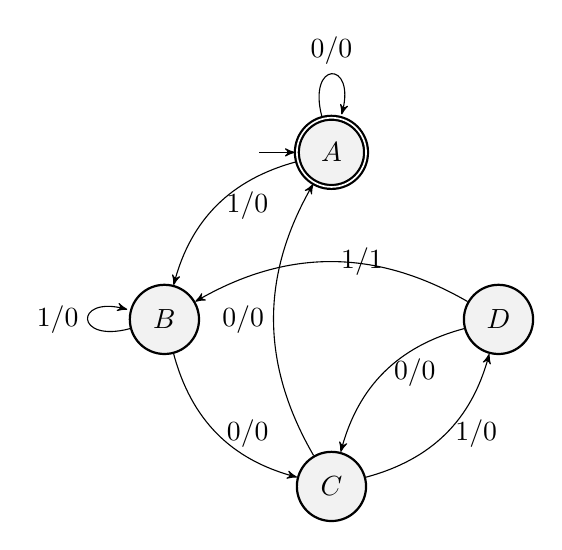
\begin{tikzpicture}
    % tikz code goes here

    \node[state, initial, accepting] (1) {$A$};
    \node[state, below left of=1] (2) {$B$};
    \node[state, below right of=2] (3) {$C$};
    \node[state, above right of=3] (4) {$D$};

    \draw (1) edge[above, bend right, right = 0.1] node{$1/0$} (2)
    (1) edge[loop above] node{$0/0$} (1)
    (2) edge[loop left] node{$1/0$} (2)
    (2) edge[below, bend right, right = 0.1] node{$0/0$} (3)
    (3) edge[left, bend left,left=0.2] node{$0/0$} (1)
    (3) edge[below, bend right, right = 0.2] node{$1/0$} (4)
    (4) edge[below, bend right, right = 0.2] node{$0/0$} (3)
    (4) edge[right, bend right, right = 0.2] node{$1/1$} (2);
        
\end{tikzpicture}


    \end{figure}
  }
  \frame{
    \frametitle{State Table for Mealy Machine Implementation}
    Generating State Table with outputs
    % Please add the following required packages to your document preamble:
% \usepackage[table,xcdraw]{xcolor}
% If you use beamer only pass "xcolor=table" option, i.e. \documentclass[xcolor=table]{beamer}
\begin{table}[]
\begin{tabular}{|c|c|c|c|}
\hline
\rowcolor[HTML]{FD6864} 
\textbf{Current State} & \textbf{Input} & \textbf{Next State} & \textbf{Output} \\ \hline
A                      & 0              & A                   & 0               \\ \hline
A                      & 1              & B                   & 0               \\ \hline
B                      & 0              & C                   & 0               \\ \hline
B                      & 1              & B                   & 0               \\ \hline
C                      & 0              & A                   & 0               \\ \hline
C                      & 1              & D                   & 0               \\ \hline
D                      & 0              & C                   & 0               \\ \hline
D                      & 1              & B                   & 1               \\ \hline
\end{tabular}
\end{table}
  }
  \frame{
    \frametitle{Simple Finite State Machine for Moore Implementation}
    \begin{figure}[!h]
    \centering
    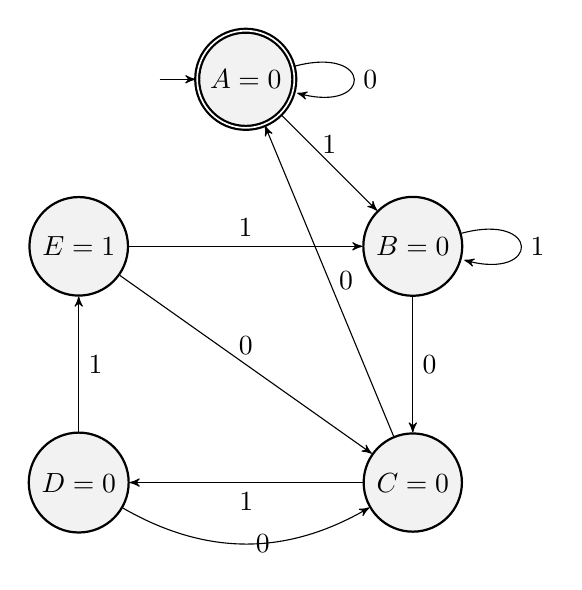
\begin{tikzpicture}
    % tikz code goes here

    \node[state, initial, accepting] (1) {$A = 0$};
    \node[state, below right of=1] (2) {$B = 0$};
    \node[state, below left of=1] (5) {$E = 1$};
    \node[state, below of=2] (3) {$C = 0$};
    \node[state, below of=5] (4) {$D = 0$};

   \draw (1) edge[above] node{$1$} (2)
   (1) edge[loop right] node{$0$} (1)
   (2) edge[loop right] node{$1$} (2)
   (2) edge[right] node{$0$} (3)
   (3) edge[right] node{$0$} (1)
   (3) edge[below] node{$1$} (4)
   (4) edge[right, bend right] node{$0$} (3)
   (4) edge[right] node{$1$} (5)
   (5) edge[above] node{$1$} (2)
   (5) edge[above] node{$0$} (3);
        
\end{tikzpicture}



    \end{figure}
  }
  \frame{
      \frametitle{State Table for Moore Machine Implementation}
      Generating State Table without outputs
      % Please add the following required packages to your document preamble:
% \usepackage[table,xcdraw]{xcolor}
% If you use beamer only pass "xcolor=table" option, i.e. \documentclass[xcolor=table]{beamer}
\begin{table}[]
\begin{tabular}{|c|c|c|}
\hline
\rowcolor[HTML]{FD6864} 
Current State & Input & Next State \\ \hline
A             & 0     & A          \\ \hline
A             & 1     & B          \\ \hline
B             & 0     & C          \\ \hline
B             & 1     & B          \\ \hline
C             & 0     & A          \\ \hline
C             & 1     & D          \\ \hline
D             & 0     & C          \\ \hline
D             & 1     & E          \\ \hline
E             & 0     & C          \\ \hline
E             & 1     & B          \\ \hline
\end{tabular}
\end{table}
  }
  \frame{
    \frametitle{Simulating Moores State Machine}
   }
\end{document}
